% move all configuration stuff into one file so we can focus on the content
\documentclass[aspectratio=169,hyperref={pdfpagelabels=false,colorlinks=true,linkcolor=white,urlcolor=lightblue},xcolor={table},t]{beamer}

%%%%%%%%%%%%%%%%%%%%%%%%%%%%%%%%%%%%%%%%%%%%%%%%%%%%%%%%%%%%%%%%%%%%%%%%%%%%%%%%%%
%%%%%%%%%%%%%%%%%%%%%%%%%%%%%%%%%%%%%%%%%%%%%%%%%%%%%%%%%%%%%%%%%%%%%%%%%%%%%%%%%%
% packages
\usepackage{pict2e}
\usepackage{epic}
\usepackage{amsmath,amsfonts,amssymb}
\usepackage{units}
\usepackage{fancybox}
\usepackage[absolute,overlay]{textpos} 
%\usepackage[table]{xcolor}
\usepackage{animate}
\usepackage{gensymb}
%\usepackage{graphicx}
%\usepackage{longtable}
\usepackage{multirow}
\usepackage{silence}
\usepackage{tikz}
\usepackage[backend=bibtex,style=ieee]{biblatex}
\AtEveryCitekey{\iffootnote{\tiny}{}}
%\addbibresource{include/references}



% fontsize
\let\Tiny=\tiny

%%%%%%%%%%%%%%%%%%%%%%%%%%%%%%%%%%%%%%%%%%%%%%%%%%%%%%%%%%%%%%%%%%%%%%%%%%%%%%%%%%
%%%%%%%%%%%%%%%%%%%%%%%%%%%%%%%%%%%%%%%%%%%%%%%%%%%%%%%%%%%%%%%%%%%%%%%%%%%%%%%%%%
% warnings
\pdfsuppresswarningpagegroup=1
\WarningFilter{biblatex}{Patching footnotes failed}
\WarningFilter{latexfont}{Font shape}
\WarningFilter{latexfont}{Some font shapes}
\WarningFilter{gensymb}{Not defining}


%%%%%%%%%%%%%%%%%%%%%%%%%%%%%%%%%%%%%%%%%%%%%%%%%%%%%%%%%%%%%%%%%%%%%%%%%%%%%%%%%%
%%%%%%%%%%%%%%%%%%%%%%%%%%%%%%%%%%%%%%%%%%%%%%%%%%%%%%%%%%%%%%%%%%%%%%%%%%%%%%%%%%
% colors
\definecolor{gtgold}{rgb}{.914, .664, 0} %0e7eed {rgb}{0.88,0.66,1,0.06} [234, 170, 0]/256 %96caff
\definecolor{darkgray}{rgb}{.15, .15, .15}
\definecolor{lightblue}{HTML}{0e7eed}
\definecolor{highlight}{rgb}{0, 0, 1} %_less!40

%%%%%%%%%%%%%%%%%%%%%%%%%%%%%%%%%%%%%%%%%%%%%%%%%%%%%%%%%%%%%%%%%%%%%%%%%%%%%%%%%%
%%%%%%%%%%%%%%%%%%%%%%%%%%%%%%%%%%%%%%%%%%%%%%%%%%%%%%%%%%%%%%%%%%%%%%%%%%%%%%%%%%
% relative paths
\graphicspath{{../graph/}}


%%%%%%%%%%%%%%%%%%%%%%%%%%%%%%%%%%%%%%%%%%%%%%%%%%%%%%%%%%%%%%%%%%%%%%%%%%%%%%%%%%
%%%%%%%%%%%%%%%%%%%%%%%%%%%%%%%%%%%%%%%%%%%%%%%%%%%%%%%%%%%%%%%%%%%%%%%%%%%%%%%%%%
% units
\setlength{\unitlength}{1mm}

%%%%%%%%%%%%%%%%%%%%%%%%%%%%%%%%%%%%%%%%%%%%%%%%%%%%%%%%%%%%%%%%%%%%%%%%%%%%%%%%%%
%%%%%%%%%%%%%%%%%%%%%%%%%%%%%%%%%%%%%%%%%%%%%%%%%%%%%%%%%%%%%%%%%%%%%%%%%%%%%%%%%%
% math
\DeclareMathOperator*{\argmax}{argmax}
\DeclareMathOperator*{\argmin}{argmin}
\DeclareMathOperator*{\atan}{atan}
\DeclareMathOperator*{\arcsinh}{arcsinh}
\DeclareMathOperator*{\sign}{sign}
\DeclareMathOperator*{\tcdf}{tcdf}
\DeclareMathOperator*{\si}{sinc}
\DeclareMathOperator*{\princarg}{princarg}
\DeclareMathOperator*{\arccosh}{arccosh}
\DeclareMathOperator*{\hwr}{HWR}
\DeclareMathOperator*{\flip}{flip}
\DeclareMathOperator*{\sinc}{sinc}
\DeclareMathOperator*{\floor}{floor}
\newcommand{\e}{{e}}
\newcommand{\jom}{\mathrm{j}\omega}
\newcommand{\jOm}{\mathrm{j}\Omega}
\newcommand   {\mat}[1]    		{\boldsymbol{\uppercase{#1}}}		%bold
\renewcommand {\vec}[1]    		{\boldsymbol{\lowercase{#1}}}		%bold

%%%%%%%%%%%%%%%%%%%%%%%%%%%%%%%%%%%%%%%%%%%%%%%%%%%%%%%%%%%%%%%%%%%%%%%%%%%%%%%%%%
%%%%%%%%%%%%%%%%%%%%%%%%%%%%%%%%%%%%%%%%%%%%%%%%%%%%%%%%%%%%%%%%%%%%%%%%%%%%%%%%%%
% media9
\newcommand{\includeaudio}[1]{
\href{run:audio/#1.mp3}{
\includegraphics[width=5mm, height=5mm]{graph/SpeakerIcon}}}

\newcommand{\includeanimation}[4]{{\begin{center}
                        \animategraphics[autoplay,loop,scale=.7]{#4}{animation/#1-}{#2}{#3}        
                        \end{center}
                        \addreference{matlab source: \href{https://github.com/alexanderlerch/ACA-Plots/blob/master/matlab/animate#1.m}{matlab/animate#1.m}}}
                        \inserticon{video}}
                        
%%%%%%%%%%%%%%%%%%%%%%%%%%%%%%%%%%%%%%%%%%%%%%%%%%%%%%%%%%%%%%%%%%%%%%%%%%%%%%%%%%
%%%%%%%%%%%%%%%%%%%%%%%%%%%%%%%%%%%%%%%%%%%%%%%%%%%%%%%%%%%%%%%%%%%%%%%%%%%%%%%%%%
% other commands
\newcommand{\question}[1]{%\vspace{-4mm}
                          \setbeamercovered{invisible}
                          \begin{columns}[T]
                            \column{.9\textwidth}
                                \textbf{#1}
                            \column{.1\textwidth}
                                \vspace{-8mm}
                                \begin{flushright}
                                     
\includegraphics[width=.9\columnwidth]{graph/question_mark}
                                \end{flushright}
                                \vspace{6mm}
                          \end{columns}\pause\vspace{-12mm}}

\newcommand{\toremember}[1]{
                        \inserticon{lightbulb}
                        }

\newcommand{\matlabexercise}[1]{%\vspace{-4mm}
                          \setbeamercovered{invisible}
                          \begin{columns}[T]
                            \column{.8\textwidth}
                                \textbf{matlab exercise}: #1
                            \column{.2\textwidth}
                                \begin{flushright}
                                     \includegraphics[scale=.5]{graph/logo_matlab}
                                \end{flushright}
                                %\vspace{6mm}
                          \end{columns}}

\newcommand{\addreference}[1]{  
                  
                    \begin{textblock*}{\baselineskip }(.98\paperwidth,.5\textheight) %(1.15\textwidth,.4\textheight)
                         \begin{minipage}[b][.5\paperheight][b]{1cm}%
                            \vfill%
                             \rotatebox{90}{\tiny {#1}}
                        \end{minipage}
                   \end{textblock*}
                    }
                    
\newcommand{\figwithmatlab}[1]{
                    \begin{figure}
                        \centering
                        \includegraphics[scale=.7]{#1}
                        %\label{fig:#1}
                    \end{figure}
                    
                    \addreference{matlab source: \href{https://github.com/alexanderlerch/MUSI-6202/blob/main/matlab/plot#1.m}{plot#1.m}}}
\newcommand{\figwithref}[2]{
                    \begin{figure}
                        \centering
                        \includegraphics[scale=.7]{#1}
                        \label{fig:#1}
                    \end{figure}
                    
                    \addreference{#2}}  
                                    
\newcommand{\inserticon}[1]{
                    \begin{textblock*}{100mm}(14.5cm,7.5cm)
                        \includegraphics[height=.8cm,keepaspectratio]{graph/#1}
                    \end{textblock*}}            

%%%%%%%%%%%%%%%%%%%%%%%%%%%%%%%%%%%%%%%%%%%%%%%%%%%%%%%%%%%%%%%%%%%%%%%%%%%%%%%%%%
%%%%%%%%%%%%%%%%%%%%%%%%%%%%%%%%%%%%%%%%%%%%%%%%%%%%%%%%%%%%%%%%%%%%%%%%%%%%%%%%%%
% counters
\newcounter{i}
\newcounter{j}
\newcounter{iXOffset}
\newcounter{iYOffset}
\newcounter{iXBlockSize}
\newcounter{iYBlockSize}
\newcounter{iYBlockSizeDiv2}
\newcounter{iXBlockSizeDiv2}
\newcounter{iDistance}

\newcommand{\IEEELink}{https://ieeexplore.ieee.org/servlet/opac?bknumber=9965970}



\subtitle{Part 4: Signal Description}

%%%%%%%%%%%%%%%%%%%%%%%%%%%%%%%%%%%%%%%%%%%%%%%%%%%%%%%%%%%%%%%%%%%%%%%%%%%%
\begin{document}
    % generate title page
	\title[]{Digital Signal Processing for Music}   
\author[alexander lerch]{alexander lerch} 
%\institute{~}
%\date[Alexander Lerch]{}
\titlegraphic{\vspace{-16mm}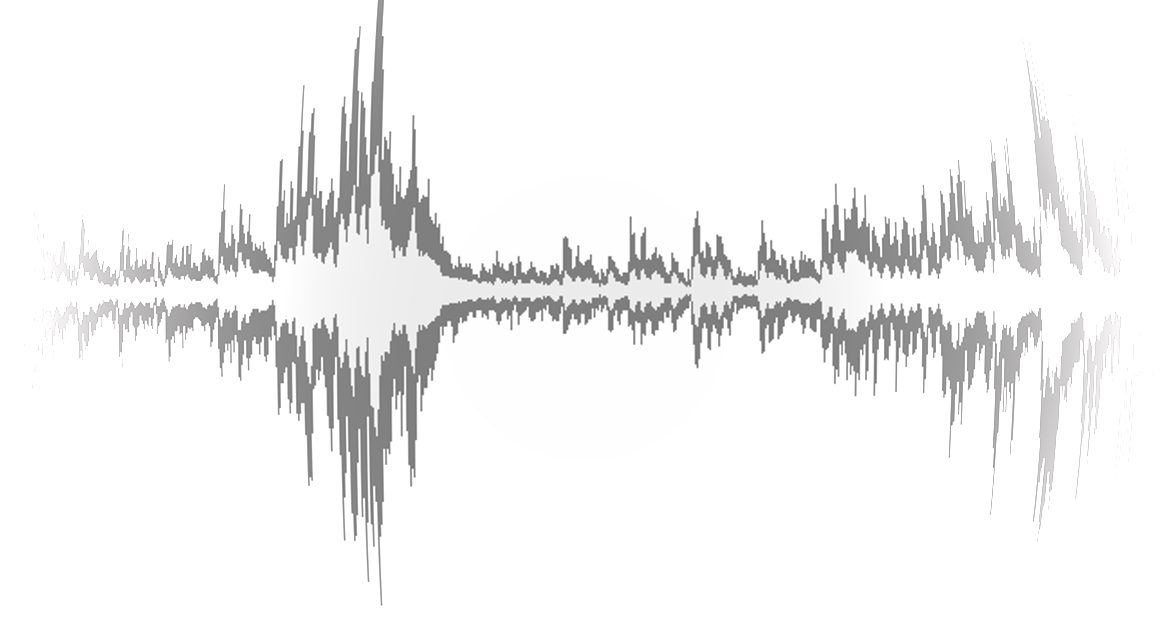
\includegraphics[width=\textwidth,height=3cm]{title}}


\begin{frame}
    \titlepage
    %\vspace{-5mm}
    \begin{flushright}
        \href{http://www.gtcmt.gatech.edu}{
\includegraphics[height=.8cm,keepaspectratio]{../shared/Logo_GTCMT_black}}
    \end{flushright}
\end{frame}


\section{introduction}
\begin{frame}{introduction}{description of (random) signals}
    \begin{itemize}
        \item   ergodic signals do not have a functional description
        \item[$\Rightarrow$]    other ways of describing these signals have to be found
        \bigskip
        \item<2->   ergodic signal characteristics are not time variant
        \item<2->[$\Rightarrow$]    we are looking for \textbf{time-independent descriptions}
        \bigskip
        \item<3-> these descriptions might also be convenient to use for some deterministic signals
    \end{itemize}
\end{frame}

\section{probability distribution}
\begin{frame}{audio signal description}{probability and occurrence}
	\begin{itemize}
		\item[]	$N$: number of overall observations
		\item[] $N(x_i)$: number of occurrences of symbol $x_i$
	\end{itemize}
	
	\pause
	\begin{itemize}
		\item	relative number of occurrences:
				\begin{equation*}
					\hat{p}_i = \frac{N(x_i)}{N}
				\end{equation*}
		
		\pause
		\item	probability:
				\begin{equation*}
					p_i = \lim\limits_{N\rightarrow\infty} \frac{N(x_i)}{N}
				\end{equation*}
	\end{itemize}
    \pause
    \begin{block}{properties}
        \begin{itemize}
            \item[]   $\sum\limits_i p_i = 1$
            \item[]   $0 \leq p_i \leq 1$
        \end{itemize}
    \end{block}
\end{frame}

\begin{frame}{audio signal description}{probability distribution example}
    \setbeamercovered{invisible}
        \begin{itemize}
            \item roll of a die
                \begin{footnotesize}
                \begin{table}
                    \centering
                        \begin{tabular}{lcccccc}
                        \textbf{value} & 1&2&3&4&5&6\\
                        \textbf{p(x)} & \nicefrac{1}{6}& \nicefrac{1}{6}& \nicefrac{1}{6}& \nicefrac{1}{6}& \nicefrac{1}{6}& \nicefrac{1}{6}
                        \end{tabular}
                \end{table}
                \end{footnotesize}
            \pause
            \bigskip
            \question {probability distribution for the roll of two dice}
            \begin{footnotesize}
            \begin{table}
                \centering
                    \begin{tabular}{lccccccccccc}
                    \textbf{value} & 2&3&4&5&6&7&8&9&10&11&12\\
                    \textbf{p(x)} & \nicefrac{1}{36}& \nicefrac{1}{18}& \nicefrac{1}{12}& \nicefrac{1}{9}& \nicefrac{5}{36}& \nicefrac{1}{6}& \nicefrac{5}{36}& \nicefrac{1}{9}& \nicefrac{1}{12}& \nicefrac{1}{18}& \nicefrac{1}{36}
                    \end{tabular}
            \end{table}
            \end{footnotesize}
            \begin{figure}
                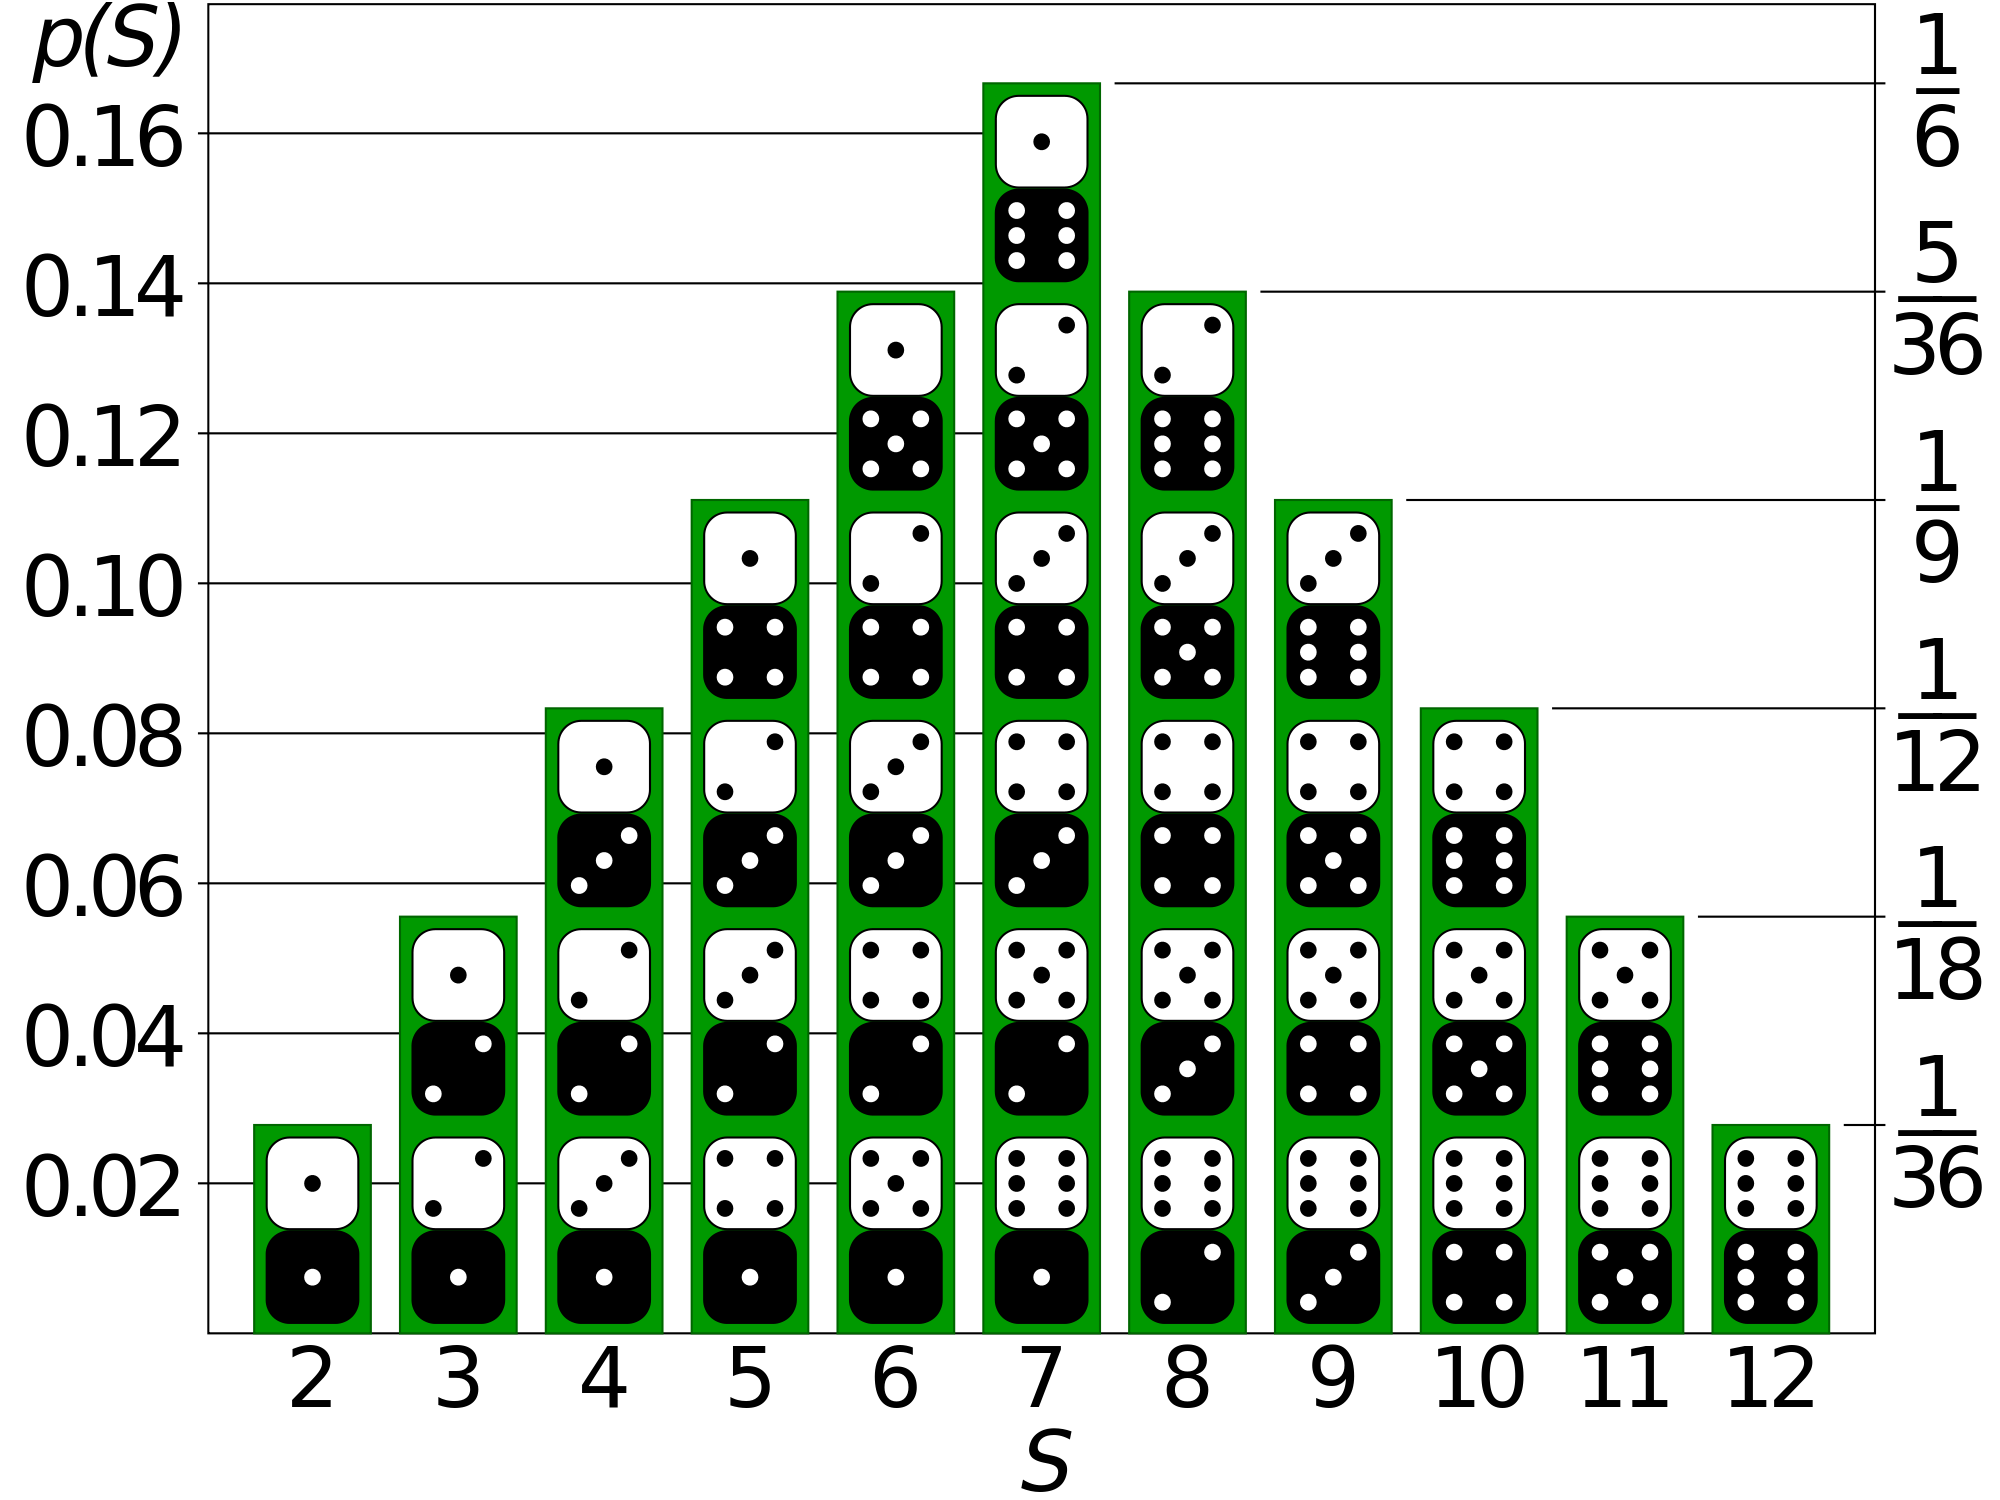
\includegraphics[scale=.06]{graph/diceprobdist}
            \end{figure}
        \end{itemize}
\end{frame}

\section{probability density function}
\begin{frame}{audio signal description}{continuous probability density distribution}
	$i\rightarrow$ continuous $\Rightarrow$ \textbf{PDF} 

	\pause
	\begin{eqnarray*}
		\int\limits_{-\infty}^{\infty} p_X(x)dx = 1\\
		0 \leq p_X(x)
	\end{eqnarray*}		

	\pause
	probability of $x$ being a value smaller than or equal $x_c$
				\begin{equation*}
					\int\limits_{-\infty}^{x_c} p_X(x)dx
				\end{equation*}		
\end{frame}	
	
\begin{frame}{audio signal description}{example PDF: Gaussian}
    \vspace{-5mm}
	\begin{equation*} \label{gaussverteilung}
		p_X(x)= \frac{1}{\sqrt{2\pi}\sigma_X}e^{-\frac{(x-\mu_X)^2}{2\sigma_X^2}}
	\end{equation*}
	\begin{figure}
		\centering
			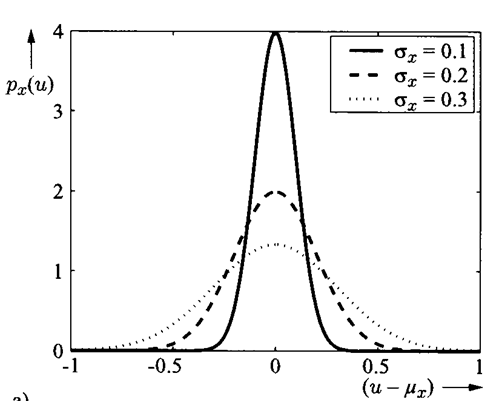
\includegraphics[scale=.5]{graph/gaussdist}
	\end{figure}
\end{frame}	

\begin{frame}{audio signal description}{example PDF: Exponential}
    \vspace{-5mm}
	\begin{equation*}
		p_X(x)= \left\lbrace  \begin{array}{ll}
		  \frac{1}{\sigma_X}e^{-\frac{x}{\sigma_X}} & x >0 \\
		  0 & \textrm{else} 
	\end{array}\right.
	\end{equation*}
    \begin{figure}
		\centering
			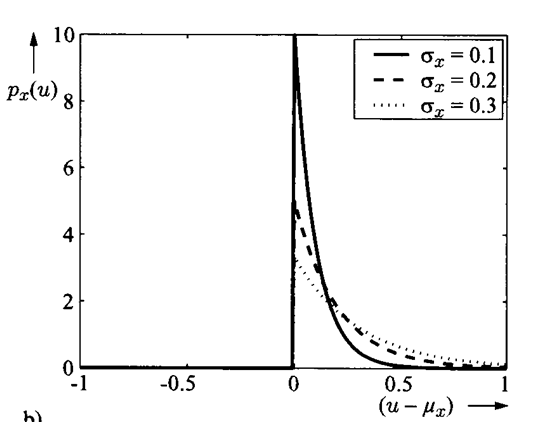
\includegraphics[scale=.5]{graph/expdist}
	\end{figure}
\end{frame}	
	
\begin{frame}{audio signal description}{example PDF: Laplace (2-sided exp)}
    \vspace{-5mm}
	\begin{equation*}
		p_X(x)= \frac{1}{\sqrt{2}\sigma_X}e^{-\sqrt{2}\frac{\mid x-\mu_X\mid}{\sigma_X}}
	\end{equation*}
	\begin{figure}
		\centering
			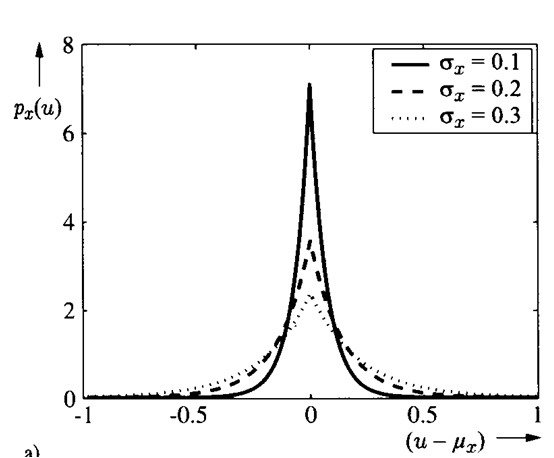
\includegraphics[scale=.5]{graph/laplacedist}
	\end{figure}
\end{frame}	

\begin{frame}{audio signal description}{measured RDF}
	\begin{figure}
		\centering
            \only<1>{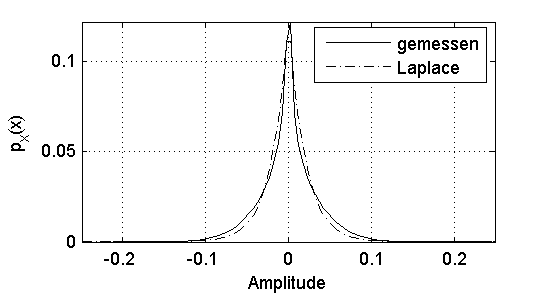
\includegraphics[scale=1.]{graph/Lerch14-9}}
            \only<2>{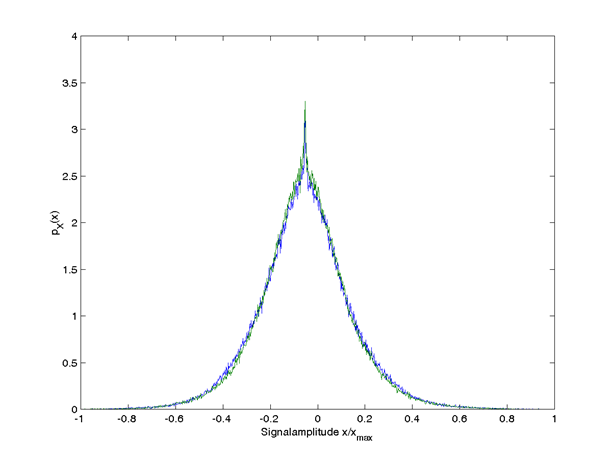
\includegraphics[scale=.5]{graph/pdf}}
	\end{figure}
\end{frame}	
	
\begin{frame}{audio signal description}{PDFs of generated signals 1/2}
    \question{describe the shape of the following PDFs}
	\begin{itemize}
		\item	white noise (uniform)
		\item	white noise (Gaussian)
		\item	DC
		\item	square
		\item	sinusoidal
		\item	sawtooth
	\end{itemize}
\end{frame}	
	
\begin{frame}{audio signal description}{distributions of generated signals 2/2}
    \vspace{-5mm}
	\begin{figure}
		\centering
			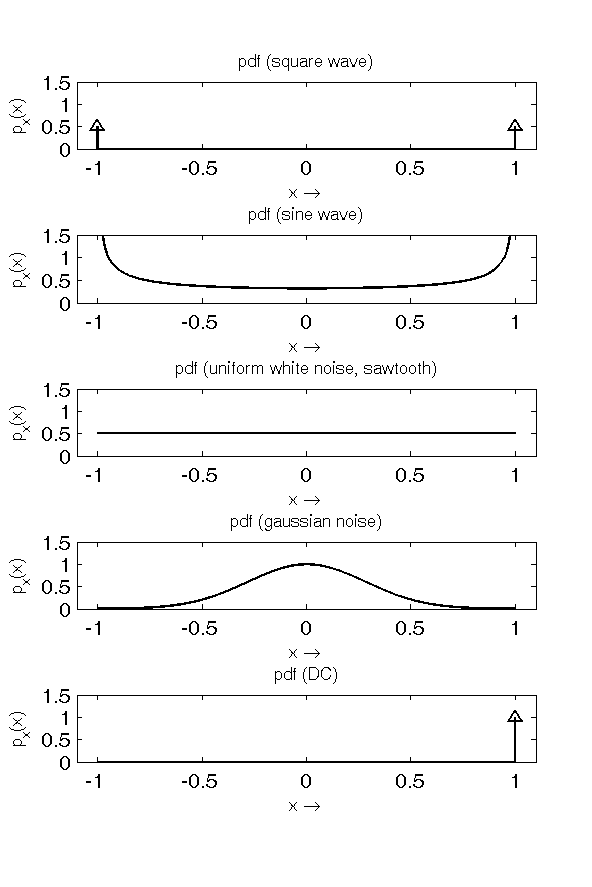
\includegraphics[scale=.5]{graph/pdfs}
	\end{figure}
\end{frame}	

\section{moments}
\begin{frame}{audio signal description}{expected value 1/3}
	Example: average grade, five students, grades: 1, 2, 1, 3, 5

	\uncover<1->{
	\begin{equation*}
		\hat{\mu}_X = \frac{1+2+1+3+5}{5} = 2.4
	\end{equation*}
	}
	\uncover<2->{
		\begin{table}[!hbt]
			\begin{center}
			\begin{footnotesize}
				\begin{tabular}{lcr}
				\hline
					\textbf{Grade} & \textbf{\# occurrences} & \textbf{relative frequency} \\
				\hline
					1	&	2	& $2/5$	\\
					2	&	1	& $1/5$	\\
					3	&	1	& $1/5$	\\
					4	&	0	& $0/5$	\\
					5	&	1	& $1/5$	\\
				\hline
				\end{tabular}  
			\end{footnotesize}
			\end{center}
		\end{table}
	}
\end{frame}		

%
%\begin{frame}{listening experiments}{descriptive analysis: metrics 1/2}
    %\begin{itemize}
        %\item   \textbf{mean}
            %\begin{itemize}
                %\item   from \textit{observations}: $\bar{x} = \frac{1}{n}\sum\limits_{i=1}^{n}{x_i}$
                %\pause
                %\item   from \textit{distribution}: $\bar{x} = \sum\limits_{\forall x}{x\cdot p(x)}$
                %\pause
                %\only<3-4>{
                %\item   simple example: 5 exam results --- 60, 40, 80, 80, 100
                    %\begin{itemize}
                        %\item   from observations: $\bar{x} = \frac{60+40+80+80+100}{5} = 72$
                        %\pause
                        %\item   from distribution
                            %\pause
                            %\begin{table}
                                %\centering
                                    %\begin{tabular}{lccccccc}
                                    %\textbf{value} & 40&50&60&70&80&90&100\\
                                    %\textbf{p(x)} & \nicefrac{1}{5}& 0 & \nicefrac{1}{5}& 0& \nicefrac{2}{5}& 0 &  \nicefrac{1}{5}
                                    %\end{tabular}
                            %\end{table}
                            %%\begin{equation*}
                                %$\bar{x} = 40\cdot\frac{1}{5} + 50\cdot\frac{0}{5} + 60\cdot\frac{1}{5} + 70\cdot\frac{0}{5} + 80\cdot\frac{2}{5} + 90\cdot\frac{0}{5} + 100\cdot\frac{1}{5} = 72$
                            %%\end{equation*}
                    %\end{itemize}
                %}
                %\pause
                %\item   5\% trimmed mean: mean without upper and lower outliers
            %\end{itemize}
        %\pause
        %\smallskip
        %\item   \textbf{variance}
            %\begin{itemize}
                %\item   from \textit{observations}: $s^2 = \frac{1}{n-1}\sum\limits_{i=1}^{n}{(x_i-\bar{x})^2}$
                %\pause
                %\item   from \textit{distribution}: $s^2 = \sum\limits_{\forall x}{(x-\bar{x})^2\cdot p(x)}$
            %\end{itemize}
        %\pause
        %\item   \textbf{standard deviation}: $s = \sqrt{s^2}$
            %\begin{itemize}
                %\item   note:\\ for normal distribution, 95\% of distribution are within $\bar{x} \pm 1.96 s$
            %\end{itemize}
    %\end{itemize}
%\end{frame}
%
%
%\begin{frame}{listening experiments}{descriptive analysis: metrics 2/2}
    %\begin{itemize}
        %\item   \textbf{skewness}
            %\begin{itemize}
                %\item   from \textit{observations}: $\gamma_1 = \frac{1}{(n-1)\cdot s^3}\sum\limits_{i=1}^{n}{(x_i-\bar{x})^3}$
                %\pause
                %\item   from \textit{distribution}: $\gamma_1 = \frac{1}{s^3}\sum\limits_{\forall x}{(x-\bar{x})^3\cdot p(x)}$
            %\end{itemize}
        %\pause
        %\item   \textbf{kurtosis}
            %\begin{itemize}
                %\item   from \textit{observations}: $\gamma_2 = \frac{1}{(n-1)\cdot s^4}\sum\limits_{i=1}^{n}{(x_i-\bar{x})^4} -3$
                %\pause
                %\item   from \textit{distribution}: $\gamma_2 = \frac{1}{s^3}\sum\limits_{\forall x}{(x-\bar{x})^3\cdot p(x)}-3$
            %\end{itemize}
        %\pause
        %\item   \textbf{percentile}: pth percentile --- p percent of observations are below this threshold
        %\pause
        %\item   \textbf{median}: 50\% percentile (``middle value of a of sorted array of all values'')
        %\pause
        %\item   \textbf{relative standard deviation} $RSD = \frac{s}{\bar{x}}$
    %\end{itemize}
    %
%\end{frame}
	

\begin{frame}{audio signal description}{expected value 2/3}
	\begin{equation*}
		\mu = \frac{2}{5}\cdot 1 + \frac{1}{5}\cdot 2 + \frac{1}{5}\cdot 3 + \frac{0}{5}\cdot 4 + \frac{1}{5}\cdot 5  = 2.4
	\end{equation*}
	
	\pause
	\begin{eqnarray*}
		\mu_X 	= \sum\limits_{\forall x} p(x)\cdot x\\
		\mu_X=\mathcal{E}\lbrace   X\rbrace  =\int\limits_{-\infty}^{+\infty}xp_X(x)dx
	\end{eqnarray*}
\end{frame}		
\begin{frame}{audio signal description}{expected value 3/3}
	generalization:
	\begin{equation*}
		\mathcal{E}\lbrace   f(X)\rbrace  = \sum\limits_i f(x)p(x)
	\end{equation*}

	\pause
	examples:
	\begin{itemize}
		\item	mean: $f(x) = x$
		\item	quad. mean: $f(x) = x^2$
	\end{itemize}
\end{frame}		

\begin{frame}{audio signal description}{(central) moments 1/2}
	\begin{itemize}
		\item	kth moment
			\begin{equation*}
				\mathcal{E}\lbrace  X^k\rbrace  = \int\limits_{-\infty}^{+\infty}x^kp_X(x)dx
			\end{equation*}
		\pause
		\item kth central moment
			\begin{equation*}
				\mathcal{E}\lbrace  (X-\mu_X)^k\rbrace  = \int\limits_{-\infty}^{+\infty}(x-\mu_X)^k p_X(x)dx
			\end{equation*}

		\pause
		\item	example: 2nd order central moment: \textbf{Variance}
			\begin{equation*}
				\sigma_X^2 = \mathcal{E}\lbrace  (X-\mu_X)^2\rbrace  = \int\limits_{-\infty}^{+\infty}(x-\mu_X)^2 p_X(x)dx
			\end{equation*}
	\end{itemize}
\end{frame}		

\begin{frame}{audio signal description}{(central) moments 2/2}
	\toremember{}
	\begin{block}{calculation of moments}
		\centering
		(central) moments (mean, power, variance, etc.) can be computed from 
		\begin{itemize}
			\item	the signal
			\item	the signal's PDF 
		\end{itemize}		
	\end{block}
\end{frame}		

\begin{frame}{audio signal description}{central moments summary}
    \begin{footnotesize}
     \begin{table}
         \centering
             \begin{tabular}{lccccc}
                 order & name & obs (cont) & pdf (cont) & \\\hline
                1 & $\mu_X$ & $\frac{1}{T}\int\limits_{-\nicefrac{T}{2}}^{\nicefrac{T}{2}} x(t)dt$ & $\int\limits_{-\infty}^{\infty}{xp_X(x)dx}$  \\
                2 & $\sigma_X^2$ & $\frac{1}{T}\int\limits_{-\nicefrac{T}{2}}^{\nicefrac{T}{2}}(x(t)-\mu_X)^2dt$ & $\int\limits_{-\infty}^{\infty} (x-\mu_X)^2p_X(x)dx$  \\
                %3 & skewness $\gamma_{X,3}$ & & $\int\limits_{-\infty}^{\infty} (x-\mu)^2p_X(x)dx$ &&\\
                %4 & kurtosis $\gamma_{X,4} & & $\int\limits_{-\infty}^{\infty} xp_X(x)dx$ &&\\
             \end{tabular}
     \end{table}
     \begin{table}
         \centering
             \begin{tabular}{lccccc}
                 order & name  & obs (disc) & pdf (disc)\\\hline
                1 & $\mu_X$         &  $\frac{1}{N}\sum\limits_{i=0}^{N} x(i)$              & $\sum\limits_{\forall x} x p(x)$ \\
                2 & $\sigma_X^2$    &  $\frac{1}{N}\sum\limits_{i=0}^{N} (x(i)-\mu_X)^2$    & $\sum\limits_{\forall x} (x-\mu_X)^2p(x)$ \\
                %3 & skewness $\gamma_{X,3}$ & & $\int\limits_{-\infty}^{\infty} (x-\mu)^2p_X(x)dx$ &&\\
                %4 & kurtosis $\gamma_{X,4} & & $\int\limits_{-\infty}^{\infty} xp_X(x)dx$ &&\\
             \end{tabular}
     \end{table}
    \end{footnotesize}
    \begin{itemize}
        \item[] standard deviation $\sigma_X = \sqrt{\sigma_X^2}$
    \end{itemize}
\end{frame}		

\section{summary}
\begin{frame}{audio signal description}{summary}
    \begin{enumerate}
        \item   PDF can tell us many important details about a signal
        \smallskip
        \item<2->   statistical measures can be used to describe signal properties
        \smallskip
        \item<3->   statistical measures can be derived from both the time domain signal and its pdf
        \smallskip
        \item<4->   often-used measures are:
            \begin{itemize}
                \item   mean and median
                \item   variance and standard deviation
                \item   higher order moments less frequently (skewness, kurtosis)
                \item   other pdf description possible (quartile-distances etc.)
            \end{itemize}
    \end{enumerate}
\end{frame}		

    
\end{document}

